\documentclass{article}
\usepackage[utf8]{inputenc}
\usepackage[slovene]{babel}
\usepackage{graphicx}
\usepackage{hyperref}
\usepackage[margin=1in]{geometry}

\title{Wikno Notes}
\date{}

\begin{document}

\maketitle

\section{Člani skupine in številka projektne skupine}
Člani: Blaž Bergant \\
Številka: 06

\section{Povezava do GitHub organizacije in repozitorijev}
\url{https://github.com/BwezB/Wikno-notes}

\section{Kratek opis projekta}
Wikno notes je inovativna aplikacija za učenje in organizacijo, ki vsem uporabnikom omogoča urejanje svojih zapiskov o skupnih entitetah in kreiranje povezav med entitetami. Vsak posameznik bo tako lahko kreiral svojo mrežo znanja (entitet z nekimi lastnostmi, ki se med seboj povezujejo), naenkrat pa si bo lahko pogledal zapiske drugih uporabnikov da razširi svoje znanje. V kontekstu organizacije, to pomeni da se bo lahko organiziral z todo listi za zasebne projekte, naenkrat pa bo projekte in todo liste lahko delil z drugimi uporabniki. 

Cilj projekta je narediti platformo, ki bo revolucionirala kako ljudje razmišljamo o zapiskih, učenju in organizaciji.

\section{Ogrodje in razvojno okolje}
\begin{itemize}
    \item Backend: Golang $\rightarrow$ Jezik je enostaven za učenje in vse bolj popularen za backende.
    \item Frontend: Swift $\rightarrow$ Z jezikom hitro zgradimo estetske aplikacije ki delujejo dobro. 
\end{itemize}

\section{Shema arhitekture}
\begin{figure}[h]
    \centering
    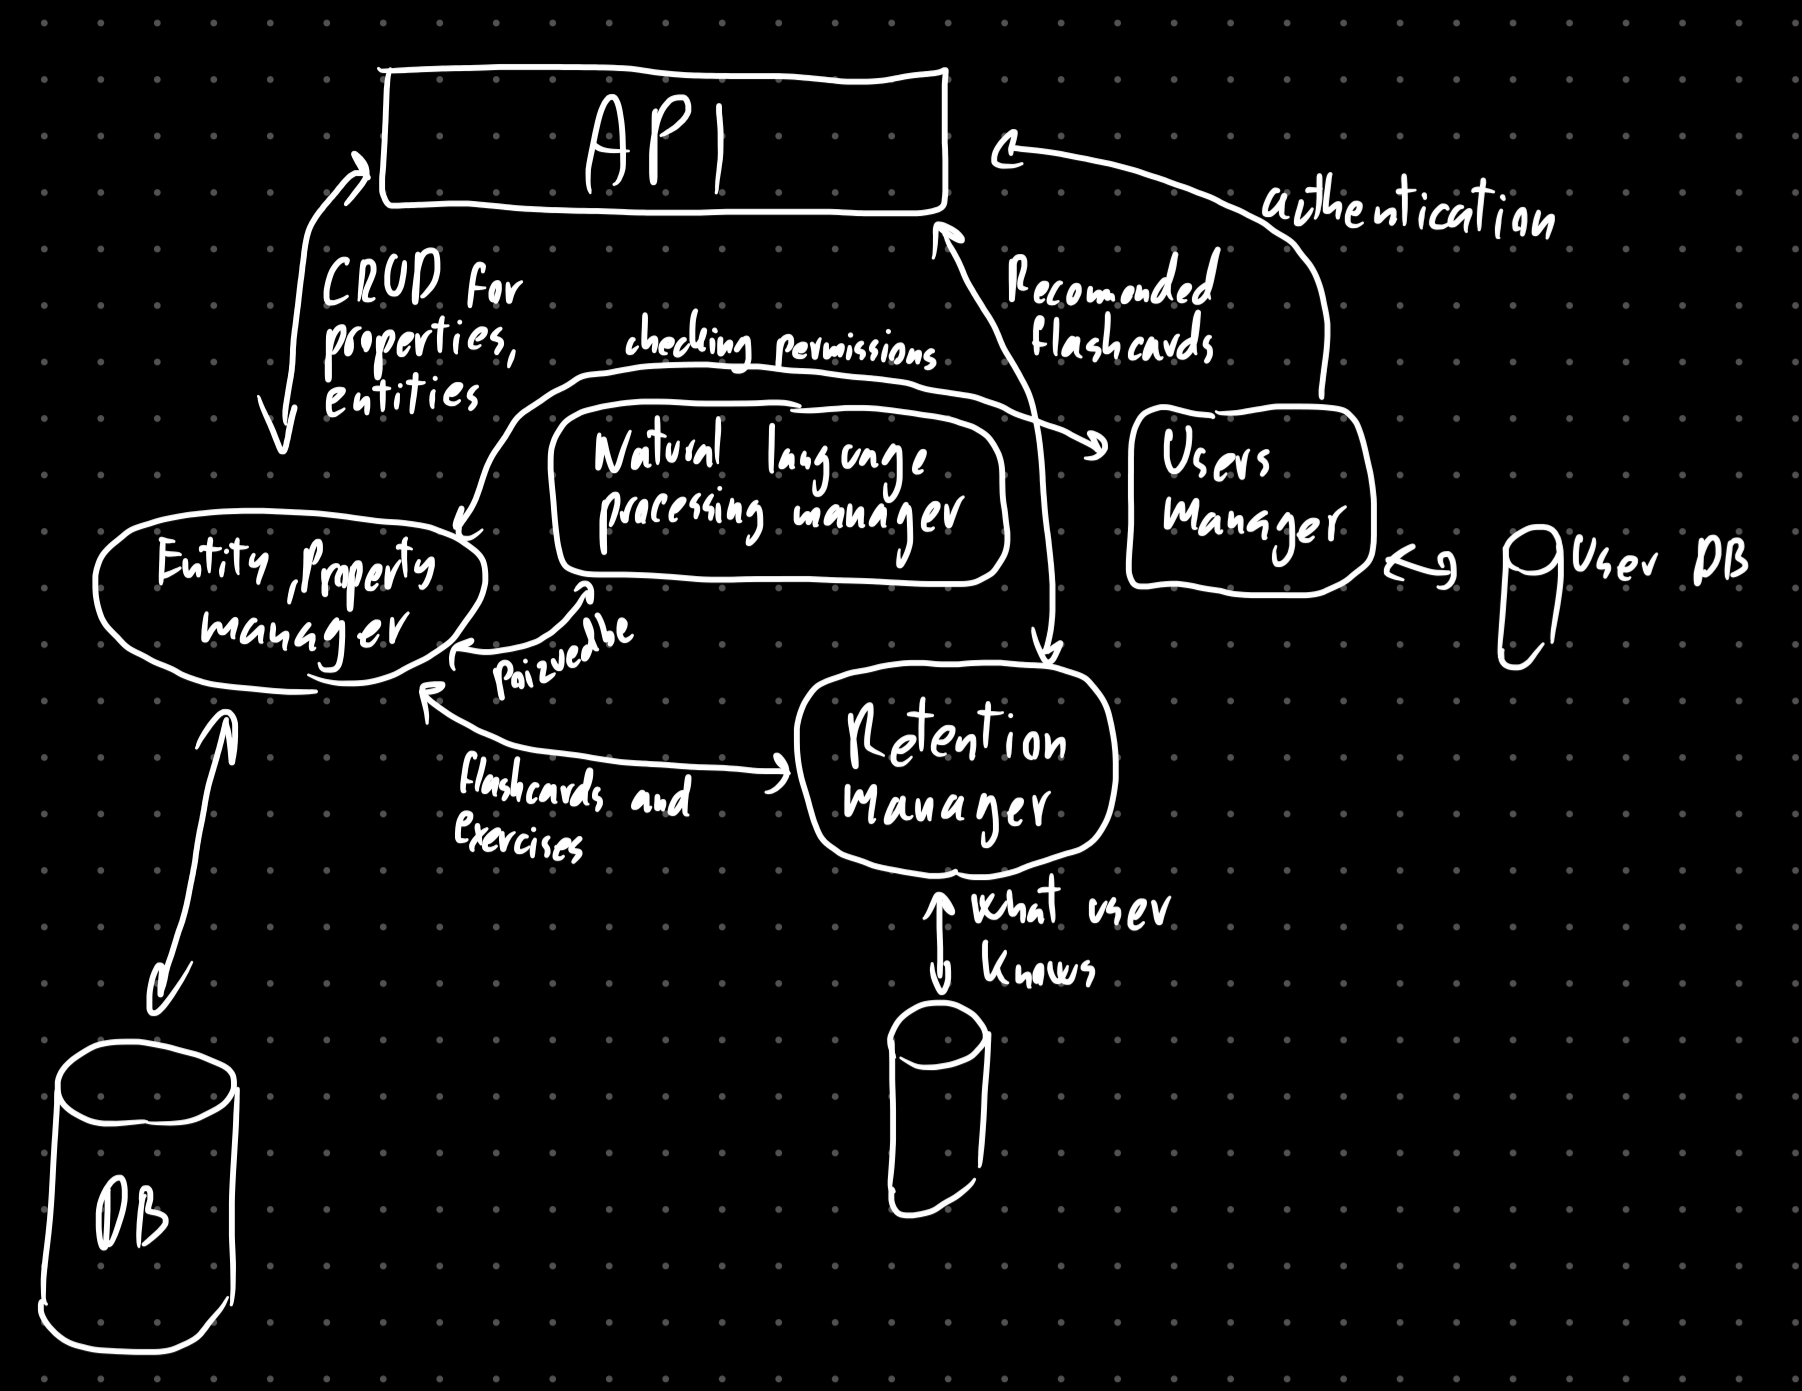
\includegraphics[width=\textwidth]{data/microservices_structure_1.png}
    \caption{Arhitektura mikrostoritev}
\end{figure}

\section{Seznam funkcionalnosti mikrostoritev}

\subsection{Entity, Property Manager}
\begin{itemize}
    \item CRUD za entitete, povezave, lastnosti.
    \item Ugotavlja duplikate v podatkih, entitetah.
    \item Pošilja in prejema vse podatke ki gredo v podatkovno bazo in iz nje
\end{itemize}

\subsection{Natural language processing Manager}
\begin{itemize}
    \item Čekira duplikate pri novo ustvarhenih tipih povezav in tipih lastnosti (če že obstaja tip z enakim pomenom)
    \item Išče kateri uporabniki delajo podobne zapiske, da jim privzeto kaže zapiske drug od drugega (ko odkrivajo novo znanje)
\end{itemize}

\subsection{Retention Manager}
\begin{itemize}
    \item Predlaga flashcarde za uporabnika (glede na že pridobljeno znanje)
    \item Predlaga vaje za uporabnika (glede na že pridobljeno znanje)
\end{itemize}

\subsection{Users Manager}
\begin{itemize}
    \item CRUD za uporabnike
    \item Avtentikacija
    \item Ali ima user pravico dobiti neke informacije
\end{itemize}

\section{Primeri uporabe}

\subsection{Kratki primeri}
\begin{enumerate}
    \item Uporabnik ustvari javno entiteto "Turingov stroj" in ji doda lastnost tipa "Opis" z vsebino "Je model računanja..."
    \item Uporabnik entiteti "Turingov stroj" doda povezavo tipa "Kreator" ki kaže na entiteto "Alan Turing"
    \item Uporabnik ustvari zasebno entiteto "Pomij posodo", z lastnostmi: Entity type: Task; Priority: A; Deadline: Today. Da se opomni o tem opravilu.
    \item Uporabnik prebere lastnosti (npr. "Opis") o entiteti "Alan Turing" od drugega uporabnika ki dela podobne zapiske kot on. 
    \item Uporabnik ustvari nov tip povezave "Tata" z opisom "Starš moški". Aplikacija ga vpraša, če je to enaka entiteta kot "Oče".
\end{enumerate}

\subsection{Kompleksni primer}

\textbf{Uporabniki:}
\begin{itemize}
    \item Ana: Ravno začela z predmetom "Algoritmi in podatkovne strukture"
    \item Bojan: Predmet "Algoritmi in podatkovne strukture" že opravil
    \item Domen: Se pripravlja na 4 rok izpita.
    \item Cvetka: Ravno začela z predmetom.
\end{itemize}

\subsubsection{Ustvarjanje in povezovanje entitet}
Ana ustvari javno entiteto "Algoritmi in podatkovne strukture" ki ji doda lastnosti in povezave:
\begin{itemize}
    \item povezava "Tip": "Predmet"
    \item povezava "Podpirajoča uztanova": "FRI"
    \item lastnost "Opis": "Predmet ki obdela osnovne algoritme in podatkovne strukture"
    \item lastnost "Semester": "3"
\end{itemize}

\subsubsection{Sodelovanje in deljenje znanja}
Bojan, ki je predmet že opravil, z napiše "Predmet se gre o časovni zahtevnosti, prostorski zahtevnosti, drevesih." in s tem kreira povezave:
\begin{itemize}
    \item povezava "Se gre o": "Časovna zahtevnost"
    \item povezava "Se gre o": "Prostorska zahtevnost"
\end{itemize}

\subsubsection{Pregled in razširitev znanja}
Domen, ki se pripravlja na izpit doda entitete povezane z ključnimi koncepti. Kreira "Rdeče črno drevo". Doda mu lastnosti:
\begin{itemize}
    \item lastnost "Kako deluje": "..."
    \item lastnost "Uporaba": "..."
    \item povezava "Je implementacija od": "Drevesa"
\end{itemize}

\subsubsection{Uporaba NLP za odkrivanje podobnosti}
Cvetka je nevešča, in kreira javno entiteto "APS", z lastnostmi in povezavami:
\begin{itemize}
    \item povezava "Tip": "Predmet"
    \item povezava "Podpirajoča uztanova": "FRI"
    \item lastnost "Semester": "3"
\end{itemize}
Ker ima entiteta podobne povezave kot že znana entiteta "Algoritmi in podatkovne strukture", "NLP Manager" predlaga da ju združi.

\subsubsection{Uporaba retention managerja}
Ana, ki se pripravlja na izpit naredi par entitet z povezavo tipa "Tip": "Flashcard", ki imajo lastnost "Vprašanje" in "Odgovor". Retention manager ji predlaga dodatne entitete tipa "Flashcard" ki so jih kreirali drugi uporabniki.

\end{document}